\documentclass[Orbiter User Manual.tex]{subfiles} 
\begin{document}

\section{Multi-functional display modes}
Multifunctional displays (or MFDs) are used in the cockpits of most military aircraft and modern airliners. The combine the function of a variety of traditional instruments in a compact format, and in combination with computerised avionics data processing they present the pilot with situation-dependent relevant data.\\
In spaceflight, providing the pilot with information appropriate to the current flight regime is even more critical, so for example the Space Shuttle made extensive use of MFD displays. Orbiter uses the MFD paradigm in a general and extendable way to provide flight data independent of vessel type (although vessel-specific MFD modes can be implemented by add-on developers).

\begin{figure}[H]
  \centering
  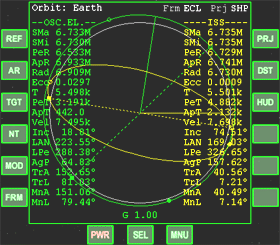
\includegraphics[width=0.5\hsize]{mfd_main.png}
\end{figure}

\noindent
The user interface of an MFD is essentially a computer display (e.g. an LED screen) and a set of input controls (usually push buttons arranged around the screen, or a separate keyboard). In Orbiter, all spacecraft MFDs work the same way, even if the specific layout varies. The picture shows the MFD representation for the generic cockpit view, which supports two MFD positions. 2D panel and virtual cockpit views may use a different number of MFD instruments.
In the centre of the MFD is the data display. The 12 buttons along the left and right edge are mode-dependent function buttons. Their labels may change according to the current operation modus of the instrument. The three buttons along the bottom edge are static and perform mode-independent system functions.\\
The MFDs can be operated either by left-clicking the buttons with the mouse, or via the keyboard. All MFD keyboard functions are \Shift-key combinations, where the left and right \Shift keys operate the left and right MFD, respectively. For instrument panels with more than two MFD displays, only two can be operated with the keyboard; the others are limited to mouse control.\\
\\
\textbf{Turning the MFD on and off}\\
The PWR button activates and deactivates the MFD display (keyboard shortcut: \Shift\keystroke{Esc}). In glass cockpit mode, turning off the MFD also hides the buttons (except the power button, so it can be turned on again).\\
\\
\textbf{Mode selection}\\
The SEL button activates the \textit{mode selection screen} (keyboard shortcut: \Ctrl\keystroke{F1}). Each MFD mode provides information for a different navigation or avionics situation (orbital parameters, surface parameters, docking and landing aids, etc.) The default modes are described below in this chapter. Many additional modes are available via 3$^{rd}$ party add-ons.\\
The mode selection screen shows the available modes in the display area, one mode next to each function button. To select a mode, simply click the corresponding button. For selection with the keyboard, press the \Ctrl key together with the mode selection key displayed in grey with each of the listed modes (for example, \Ctrl\keystroke{O} for Orbit mode).

\begin{figure}[H]
  \centering
  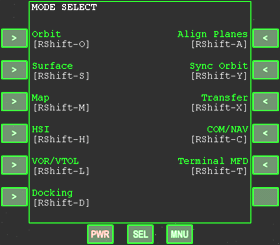
\includegraphics[width=0.5\hsize]{mfd_mode.png}
\end{figure}

\noindent
If there are more modes than can be displayed in a single page, pressing SEL (or \Ctrl\keystroke{F1}) repeatedly cycles through all mode pages. Pressing SEL on the last mode page returns to the previously selected MFD mode. Note that mode selection with keyboard shortcuts works from any of the mode selection pages, even if the requested mode is not displayed on the current page.\\
\\
\textbf{Function buttons}\\
The function of the buttons to the left and right of the display depends on the current MFD mode, and their labels change accordingly. Functions and user interface for the standard MFD modes are described below. For modes provided by 3$^{rd}$ party add-ons, consult the accompanying documentation. In some cases the buttons may act as switches, where each press executes a discrete operation. In other cases it may be necessary to press down a button continuously to adjust a parameter.

\begin{figure}[H]
  \centering
  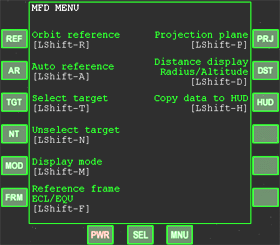
\includegraphics[width=0.5\hsize]{mfd_menu.png}
\end{figure}

\noindent
Function buttons for the two main MFD instruments can also be activated with \Ctrl-key combinations. On pressing the MNU button below the bottom edge of the screen (keyboard shortcut: \Ctrl\keystroke{`}) a short description of all function buttons for this mode is displayed, together with the keyboard shortcuts to activate them. Pressing MNU again, or pressing a function button, restores the display.\\
In glass cockpit view, and in most instrument panels in Orbiter, each MFD has 12 function buttons, but individual spacecraft can adopt a different layout in their panels. If an MFD mode assigns more function buttons than are physically present, pressing MNU repeatedly cycles through the available function pages.\\
\\
\textbf{Colour customisation}\\
The default colour schemes for MFD displays can be modified by editing the Config\textbackslash MFD\textbackslash default.cfg text file. Note that some add-on MFD Modes may define their own colour scheme which cannot be customised.


\subsection{NAV receiver/transmitter setup}
The \textit{COM/NAV setup} MFD mode provides an interface to the ship’s navigation radio receivers which feed data into the navigation instruments. It also allows to select the frequency of the ship’s long-range transponder which sends a signal identifying the vessel and its position. The mode is activated via the COM/NAV entry from the MFD mode selection page (shortcut: \Ctrl\keystroke{,} + \Ctrl\keystroke{.}).\\
\\
\textbf{Key options:}

%\begin{table}[H]
	%\centering
	\begin{longtable}{ |p{0.15\textwidth}|p{0.15\textwidth}|p{0.6\textwidth}| }
	\hline\rule{0pt}{2ex}
	\textbf{Button} & \textbf{Shortcut} & \textbf{Action}\\
	\hline\rule{0pt}{2ex}
	SL- & \Shift\keystroke{,} & Move selection up\\
	\hline\rule{0pt}{2ex}
	SL+ & \Shift\keystroke{.} & Move selection down\\
	\hline\rule{0pt}{2ex}
	<{}< & \Shift\keystroke{-} & Step frequency down 1 MHz\\
	\hline\rule{0pt}{2ex}
	>{}> & \Shift\keystroke{=} & Step frequency up 1 MHz\\
	\hline\rule{0pt}{2ex}
	< & \Shift\keystroke{[} & Step frequency down 0.05 MHz\\
	\hline\rule{0pt}{2ex}
	> & \Shift\keystroke{]} & Step frequency up 0.05 MHz\\
	\hline\rule{0pt}{2ex}
	SC< & \Shift\keystroke{Z} & Scan frequency downward\\
	\hline\rule{0pt}{2ex}
	SC> & \Shift\keystroke{X} & Scan frequency upward\\
	\hline
	\end{longtable}
%\end{table}

\noindent
\textbf{MFD control layout:}

\begin{figure}[H]
  \centering
  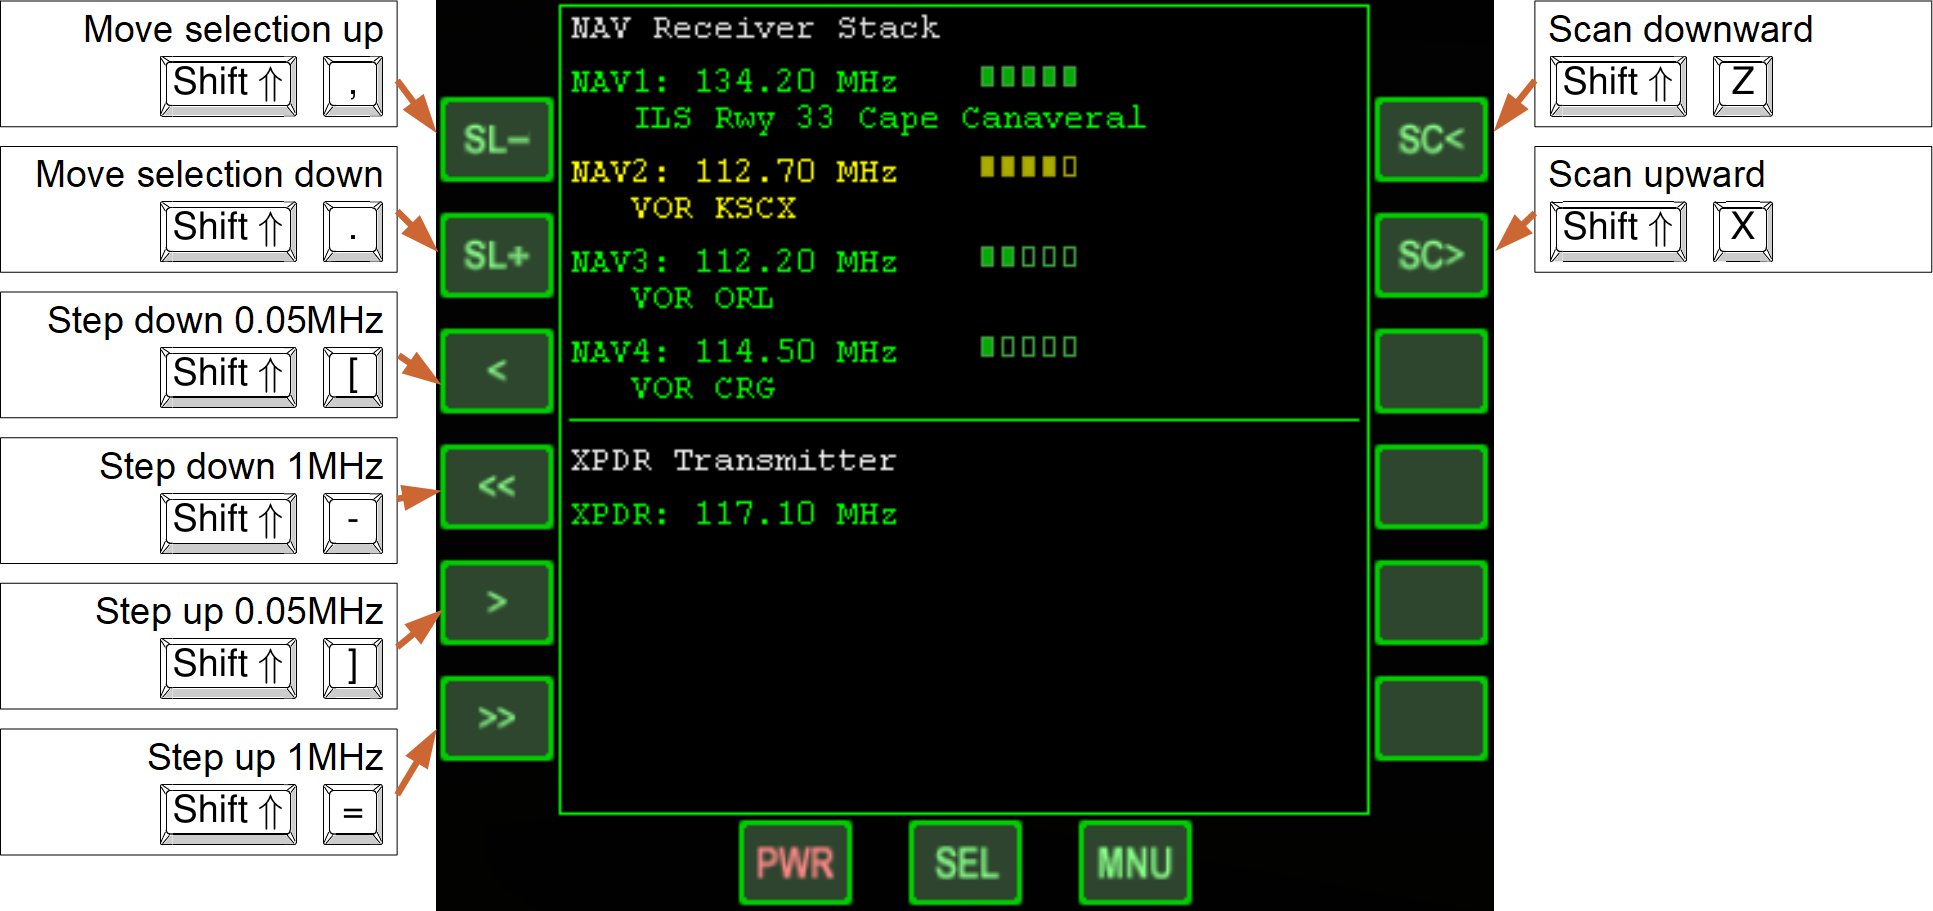
\includegraphics[width=0.99\hsize]{nav_input.png}
\end{figure}

\noindent
\textbf{MFD display components:}\\
The top part of the MFD display shows the NAV radio receiver stack. For each available receiver, the current frequency setting is shown, together with an identification of the received signal (if any) and a field strength indicator. The lower part of the display shows the transponder (XPDR) frequency.\\
The currently selected entry is highlighted in yellow. The selection can be moved up and down with the SL- (or \Shift\keystroke{,}) and SL+ (or \Shift\keystroke{.}) buttons.\\
The frequency of the selected receiver or transmitter can be tuned in steps of 1 MHz with \Shift\keystroke{-} and  \Shift\keystroke{=}, and in steps of 0.05 MHz with \Shift\keystroke{[} and \Shift\keystroke{]}, in the range from 108.00–140.00 MHz. You can sweep the frequency range down or up with \Shift\keystroke{Z} and \Shift\keystroke{X} until a signal is detected. If a compatible NAV transmitter is within range, the instrument displays information about the signal source and strength.

\begin{figure}[H]
  \centering
  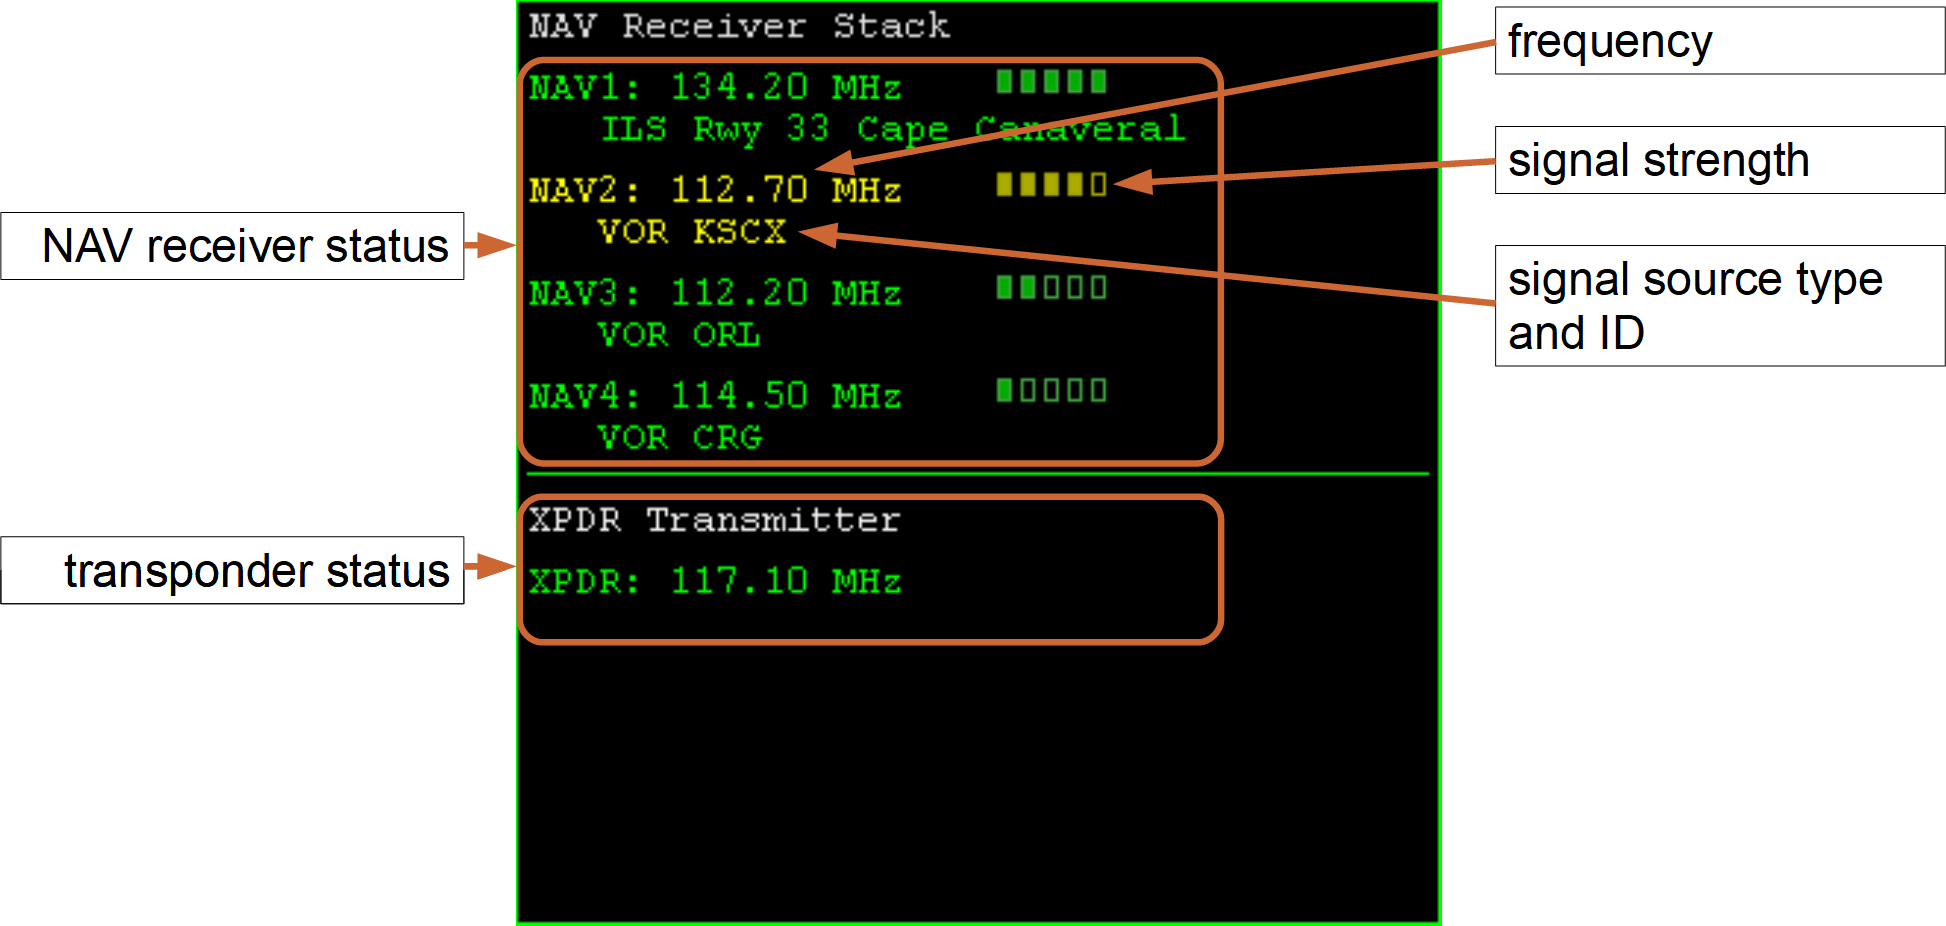
\includegraphics[width=0.99\hsize]{nav_layout.png}
\end{figure}

\noindent
In Orbiter, NAV transmitter types include VOR (VHF omnidirectional range), ILS (instrument landing system) for runway approaches and VTOL (vertical take-off and landing) pads, XPDR (vessel transponders) and IDS (instrument docking system). Each transmitter type provides information which can be fed to other MFD modes or avionics instrumentation to provide situational awareness to the pilot.\\
%TODO add section link
The \textit{Object info} (\Ctrl\keystroke{I}, see TODO) and \textit{Map} (\Ctrl\keystroke{M}, see TODO) windows are useful tools to obtain surface or vessel-based transmitter frequencies.

\begin{figure}[H]
  \centering
  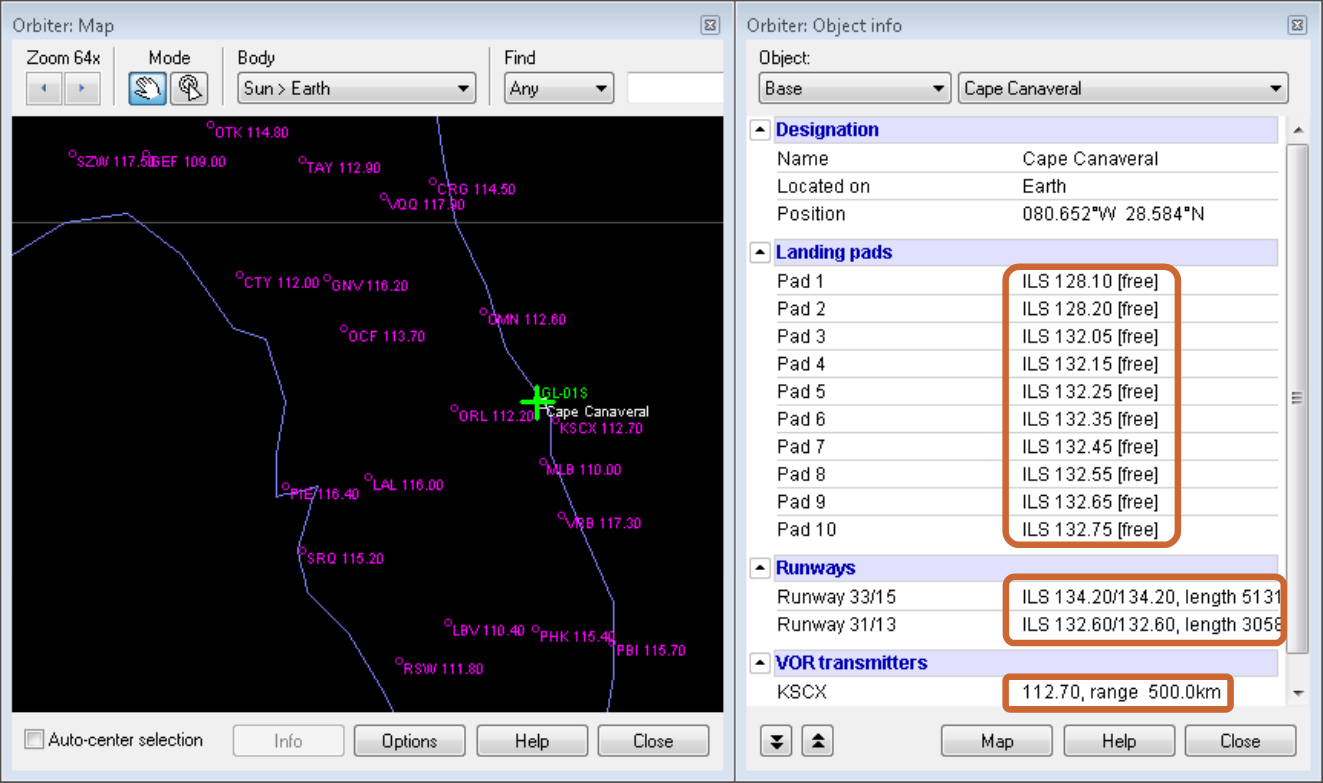
\includegraphics[width=0.75\hsize]{freq_map_info.png}
  \caption{Map window (left) and object info dialog (right) with NAV transmitter information}
\end{figure}

\noindent
The positions and frequencies of VOR stations in your vicinity can also be displayed directly in the simulation window via the VOR Markers option in the \textit{Visual helpers} dialog box (\Ctrl\keystroke{F9}).


\subsection{Surface}
The \textit{Surface} MFD mode provides avionics data useful in flight situations close to planetary surfaces. It contains an attitude indicator (artificial horizon) displaying the vessel’s attitude relative to the local horizon plane, various tapes for altitude, speed and acceleration readouts, as well as position, pressure and temperature data.\\
\\
\textbf{Key options:}

%\begin{table}[H]
	%\centering
	\begin{longtable}{ |p{0.15\textwidth}|p{0.15\textwidth}|p{0.6\textwidth}| }
	\hline\rule{0pt}{2ex}
	\textbf{Button} & \textbf{Shortcut} & \textbf{Action}\\
	\hline\rule{0pt}{2ex}
	IAS & \Shift\keystroke{I} & Switch speed readout to indicated airspeed\\
	\hline\rule{0pt}{2ex}
	TAS & \Shift\keystroke{T} & Switch speed readout to true airspeed\\
	\hline\rule{0pt}{2ex}
	GS & \Shift\keystroke{G} & Switch speed readout to ground-relative speed\\
	\hline\rule{0pt}{2ex}
	OS & \Shift\keystroke{O} & Switch speed readout to orbital speed\\
	\hline\rule{0pt}{2ex}
	HUD & \Shift\keystroke{H} & Set HUD to Surface mode\\
	\hline
	\end{longtable}
%\end{table}

\noindent
\textbf{MFD control layout:}

\begin{figure}[H]
  \centering
  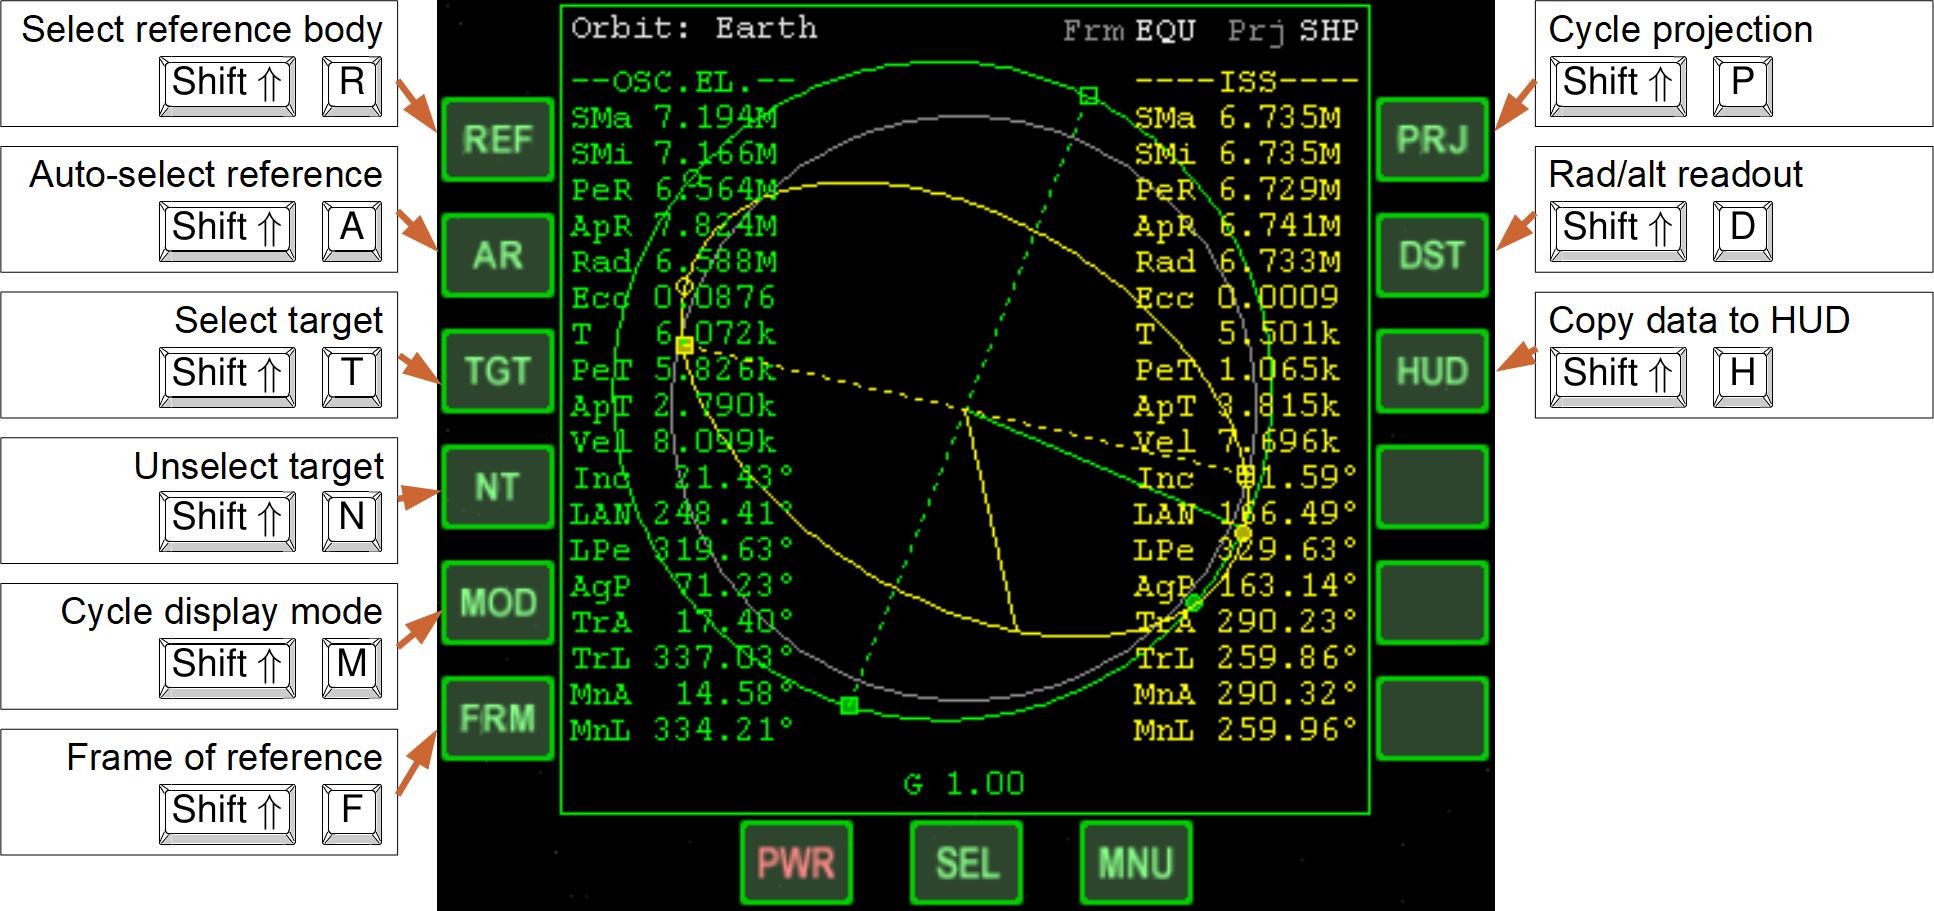
\includegraphics[width=0.75\hsize]{orbit_input.png}
\end{figure}

\noindent
\textbf{MFD display components:}\\
The display contains an attitude indicator (AI) with horizon line and pitch ladder indicating pitch and bank attitude (including numerical readouts). Above is a compass ribbon with a heading readout. To the left of the AI is the speed readout which can be set to different modes with the MFD buttons:

\begin{itemize}
\item TAS (true airspeed): The speed of the spacecraft relative to the surrounding atmosphere. Airspeed is usually measured with a pitot tube in the airstream recording the difference between free-stream and stagnation point pressure. The TAS mode is only available if the free-stream pressure $p_{1}$ > 10$^{-3}$ Pa (on Earth, this corresponds to approx. 140 km altitude). If TAS cannot be measured, the speed tape is reset to 0 and the readout shows "-{}-{}-{}-".
\item IAS (indicated airspeed): Commonly used in conventional aircraft. IAS is calibrated to atmospheric density and speed of sound at sea level. IAS and TAS are similar at low altitude, but start to diverge at higher altitudes, with IAS < TAS. The limit $p_{1}$ > 10$^{-3}$ Pa also applies to IAS availability.
\item GS (ground-relative speed): The magnitude of the vessel’s velocity vector in the rotating planet reference frame. This is similar to TAS at lower altitudes, but diverges at higher altitudes. Usually, TAS is no longer available where the differences would become significant. \textit{Note:} for an object in geostationary orbit, GS would be zero since it is stationary relative to the rotating planet frame.
\item OS (orbital speed): The magnitude of the vessel’s velocity relative to the planet’s centre in a non-rotating frame. This is identical to the Vel readout in the \textit{Orbit} MFD. Note: OS is usually non-zero for a vessel at rest on the planet surface, because the planet itself is rotating.
\end{itemize}

\begin{figure}[H]
  \centering
  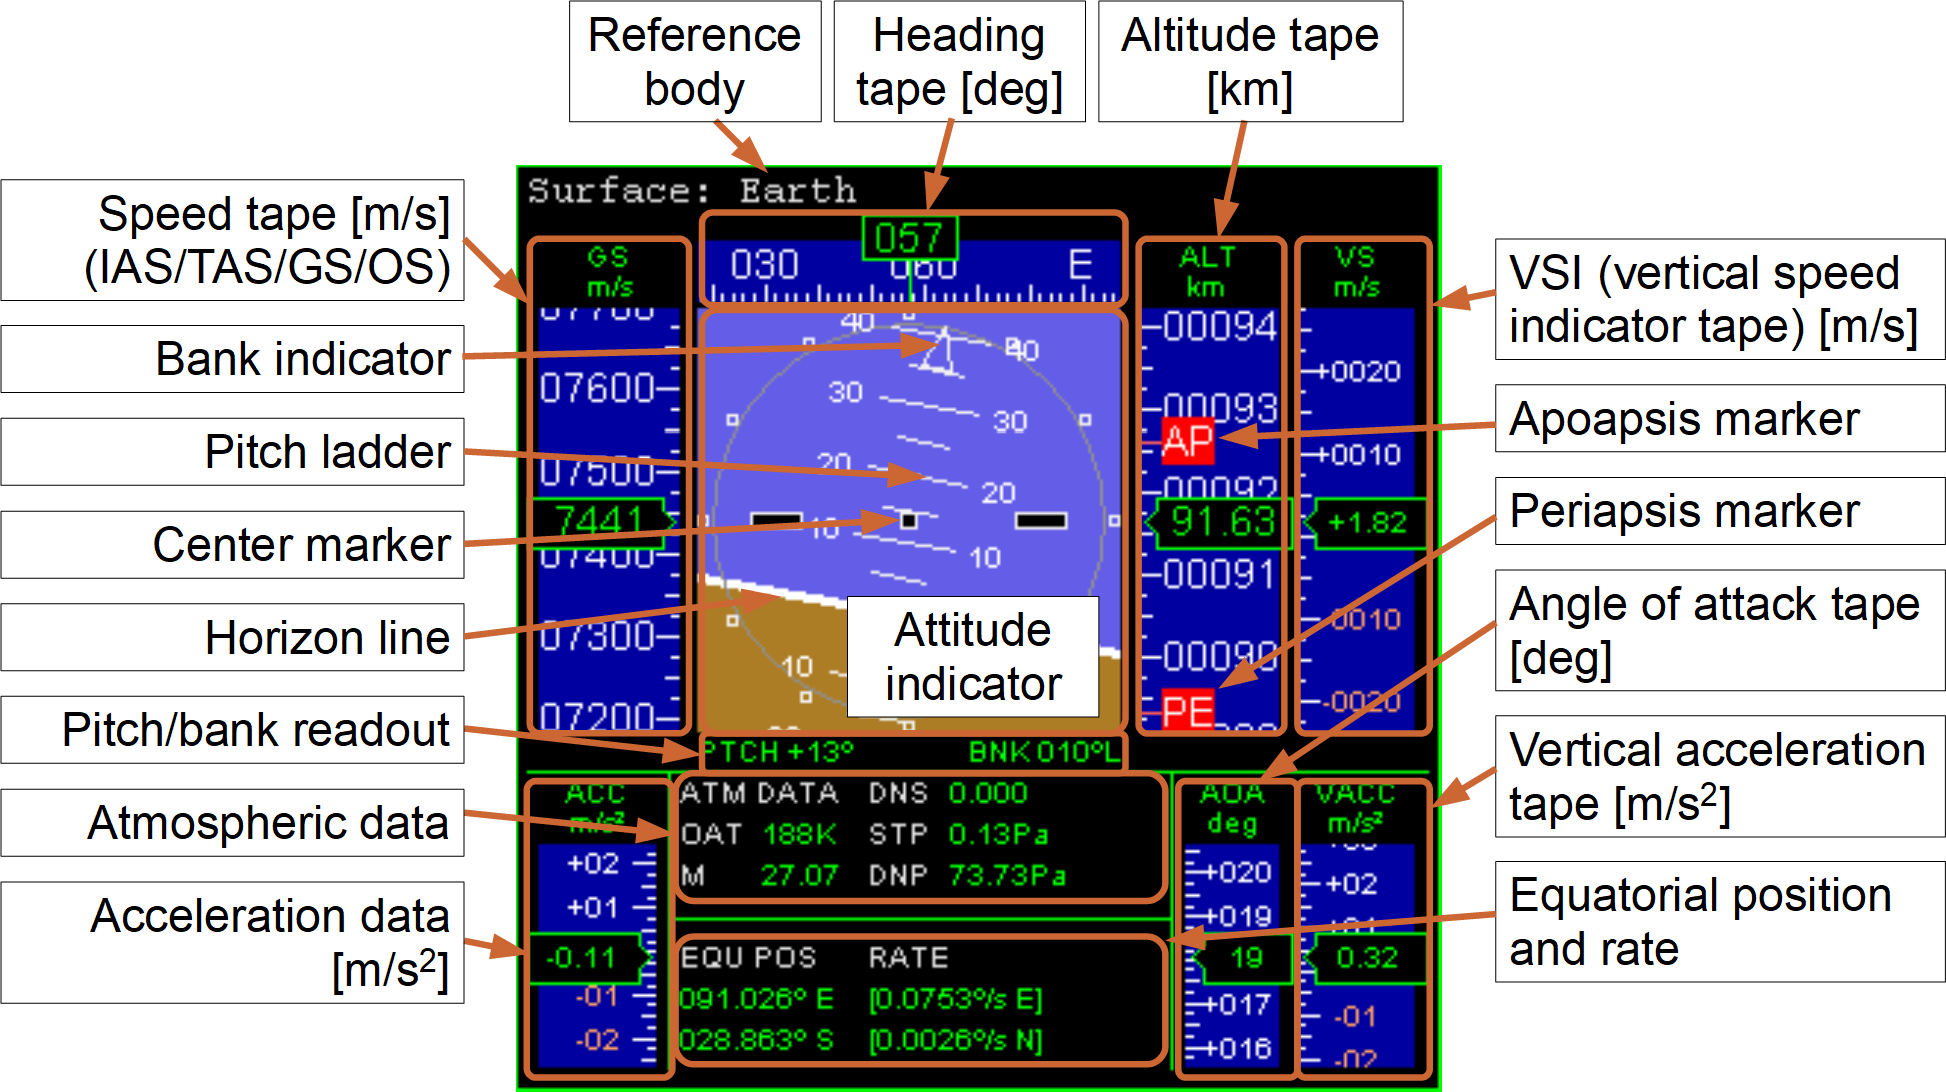
\includegraphics[width=0.99\hsize]{orbit_layout.png}
\end{figure}

\noindent
To the right of the IA is the altitude tape showing the vessel altitude [km] above the surface (ALT-R) at altitudes < 10 km, or altitude above mean planet radius (ALT) otherwise. To the right of the altitude tape is the vertical speed tape (VS) [m/s].\\
In the lower part of the display are the acceleration tape (ACC) [m/s$^{2}$] (left), and the AOA (angle of attack) and vertical acceleration (VACC) [m/s$^{2}$] tapes (right).\\
Below the AI are atmospheric data readouts: atmospheric density (DNS), static pressure (STP), dynamic pressure (DNP), outside air temperature (OAT) and Mach number (M). In the block below are vessel’s equatorial position (longitude, latitude) [deg] and their rates [deg/s].


\subsection{Map}
%TODO add section link
The \textit{Map} MFD mode shows the surface of a celestial body in a cylindrical projection, including coastlines and contour lines. It can display surface markers for bases and VOR beacons, as well as ground tracks or orbital plane intersections for objects orbiting the body. The display elements are similar to the \textit{Map} dialog (see TODO).\\
\\
\textbf{Key options (map view):}

%\begin{table}[H]
	%\centering
	\begin{longtable}{ |p{0.15\textwidth}|p{0.15\textwidth}|p{0.6\textwidth}| }
	\hline\rule{0pt}{2ex}
	\textbf{Button} & \textbf{Shortcut} & \textbf{Action}\\
	\hline
	\multicolumn{3}{|c|}{\rule{0pt}{2ex}\textbf{\textit{Map view:}}}\\
	\hline\rule{0pt}{2ex}
	REF & \Shift\keystroke{R} & Select a celestial body for map display\\
	\hline\rule{0pt}{2ex}
	TGT & \Shift\keystroke{T} & Select a target object\\
	\hline\rule{0pt}{2ex}
	ZM- & \Shift\keystroke{X} & Zoom out by factor 2 down to 1x (global view)\\
	\hline\rule{0pt}{2ex}
	ZM+ & \Shift\keystroke{Z} & Zoom in by factor 2 up to 128x (2.8° x 2.8° cover)\\
	\hline\rule{0pt}{2ex}
	TRK & \Shift\keystroke{K} & Toggle automatic vessel track mode on/off\\
	\hline\rule{0pt}{2ex}
	DSP & \Shift\keystroke{D} & Display parameter configuration page\\
	\hline\rule{0pt}{2ex}
	UP & \Shift\keystroke{-} & Scroll map display up (disabled in track mode)\\
	\hline\rule{0pt}{2ex}
	DN & \Shift\keystroke{=} & Scroll map display down (disabled in track mode)\\
	\hline\rule{0pt}{2ex}
	< & \Shift\keystroke{[} & Scroll map display left (disabled in track mode)\\
	\hline\rule{0pt}{2ex}
	> & \Shift\keystroke{]} & Scroll map display right (disabled in track mode)\\
	\hline
	\multicolumn{3}{|c|}{\rule{0pt}{2ex}\textbf{\textit{Parameter selection view:}}}\\
	\hline\rule{0pt}{2ex}
	UP & \Shift\keystroke{-} & Move selection marker up\\
	\hline\rule{0pt}{2ex}
	DN & \Shift\keystroke{=} & Move selection marker down\\
	\hline\rule{0pt}{2ex}
	MOD & \Shift\keystroke{M} & Modify the currently selected option\\
	\hline\rule{0pt}{2ex}
	OK & \Shift\keystroke{O} & Return to map view\\
	\hline
	\end{longtable}
%\end{table}

\noindent
\textbf{MFD control layout:}

\begin{figure}[H]
  \centering
  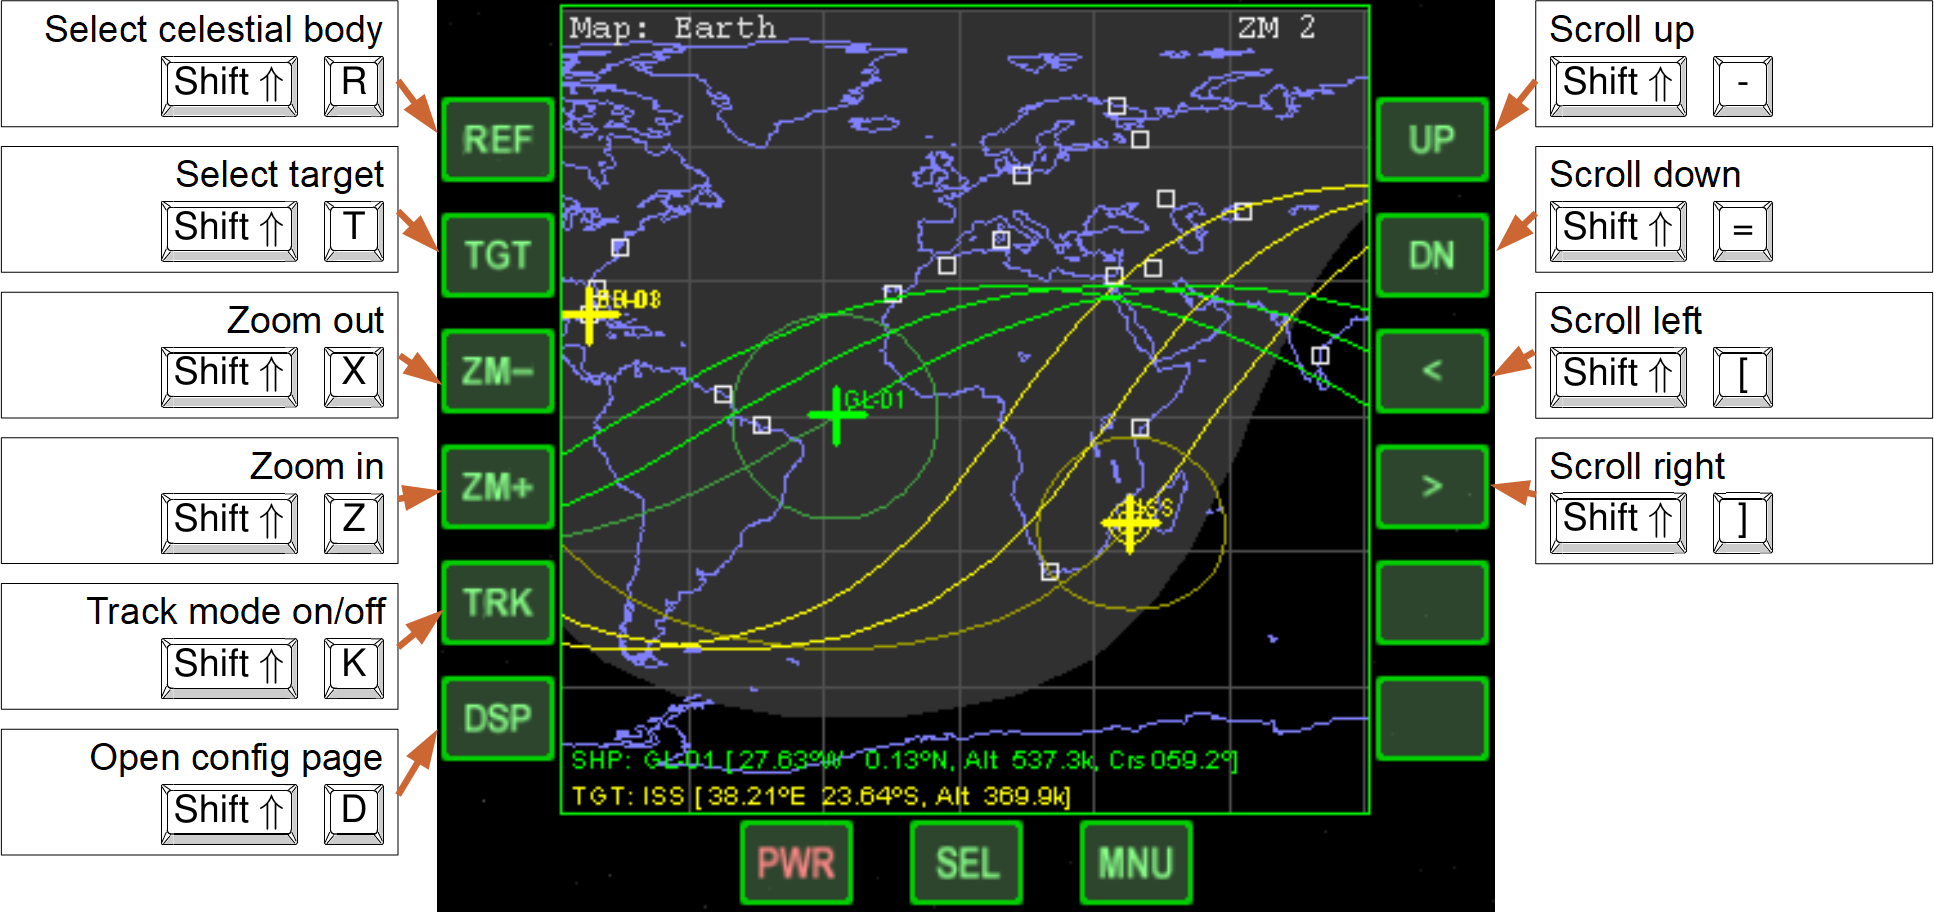
\includegraphics[width=0.99\hsize]{map_input.png}
\end{figure}

\noindent
\textbf{MFD display components:}\\
The map display elements include:

\begin{itemize}
\item Current position (green +) projected onto the planet surface.
\item Positions of any other spacecraft currently located on the planet surface or orbiting the planet (yellow +)
\item Orbit ground track (past and predicted for a few orbits), or alternatively orbit plane (the great circle defined by the intersection of the orbital plane with the planet surface)
\item Horizon line: indicates the limit of visibility of the planet surface as seen from the current vessel position (or equivalently, the area of the planet surface from which the spacecraft would appear above the horizon for a ground-based observer).
\item Terminator line: indicates the lit hemisphere of the planet with a boundary line and/or a shaded area.
\item Coastlines and contour lines (e.g. topographical levels) where supported.
\item Location of surface bases, VOR transmitters with frequencies and other surface features (cities or geological features)
\item The current position (longitude, latitude, altitude) and course of the vessel, and the position data of an optional target object or surface base are shown at the bottom of the screen. If the target is a base, distance and bearing from the current vessel position are also displayed.
\end{itemize}

\noindent
The map can be zoomed and scrolled. It is also possible track the current position (which disables manual scrolling). At high zoom levels, labels for marked surface features are shown.

\begin{figure}[H]
  \centering
  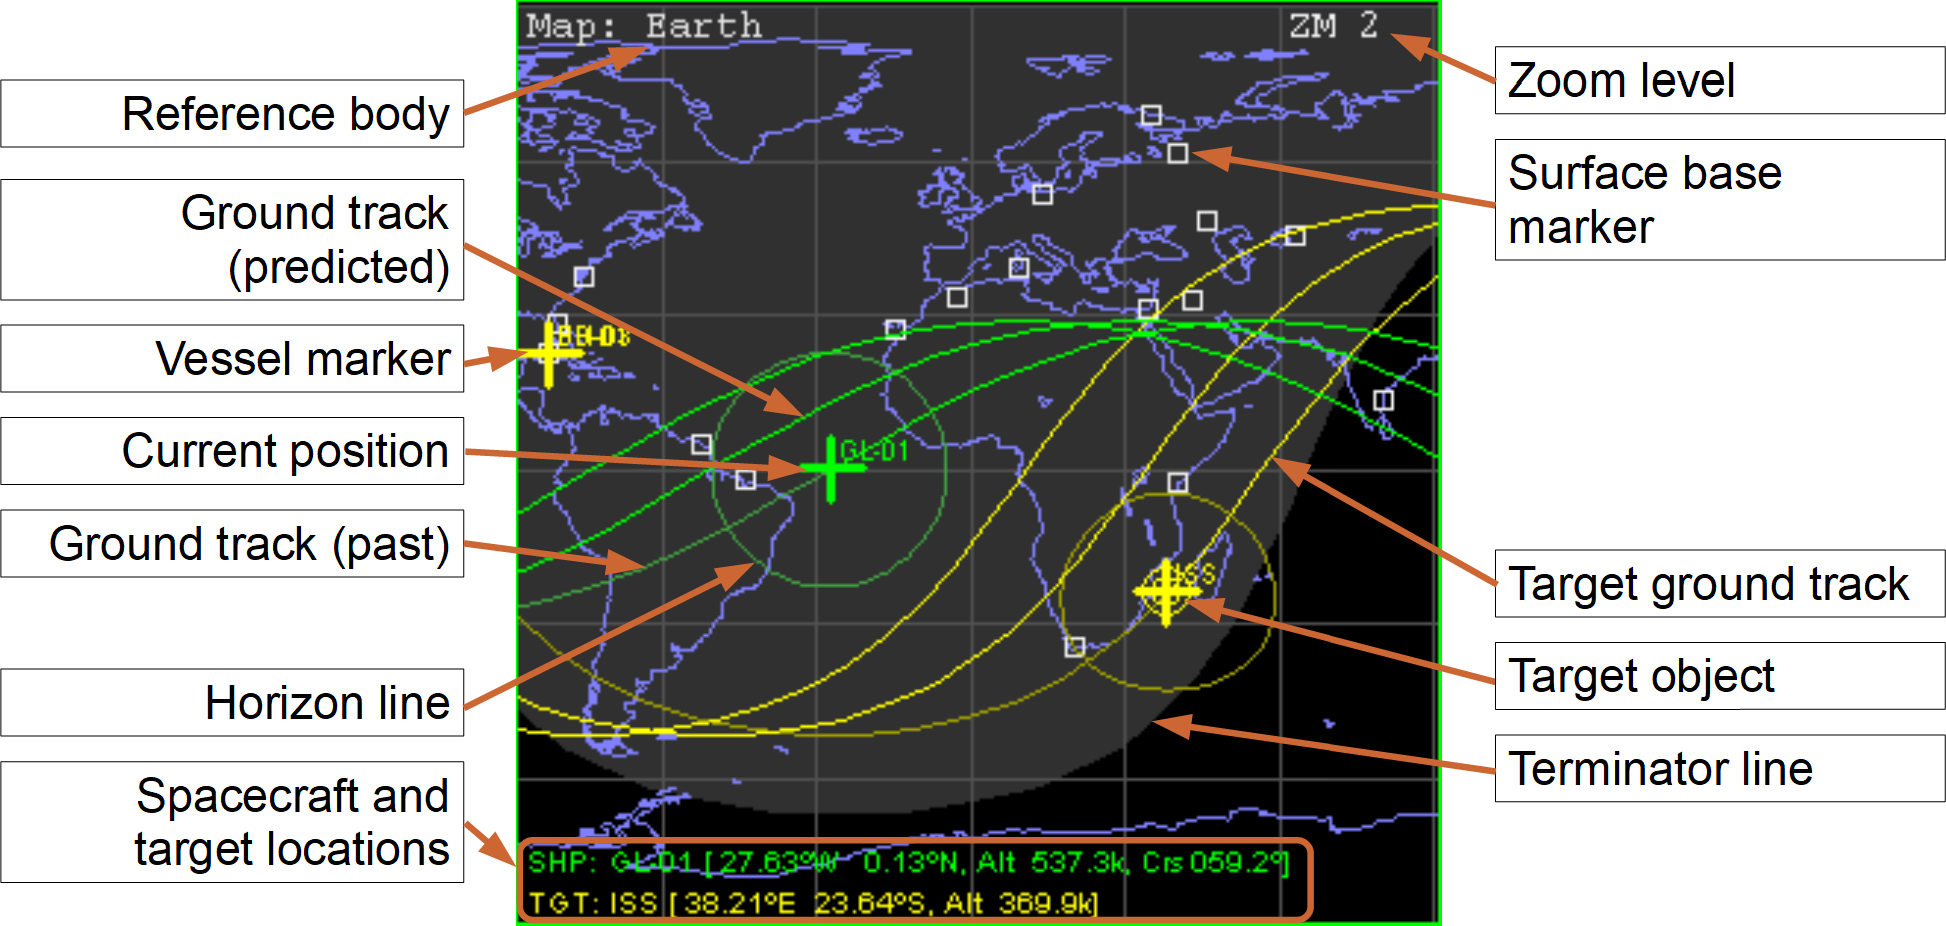
\includegraphics[width=0.99\hsize]{map_layout_1.png}
\end{figure}

\begin{figure}[H]
  \centering
  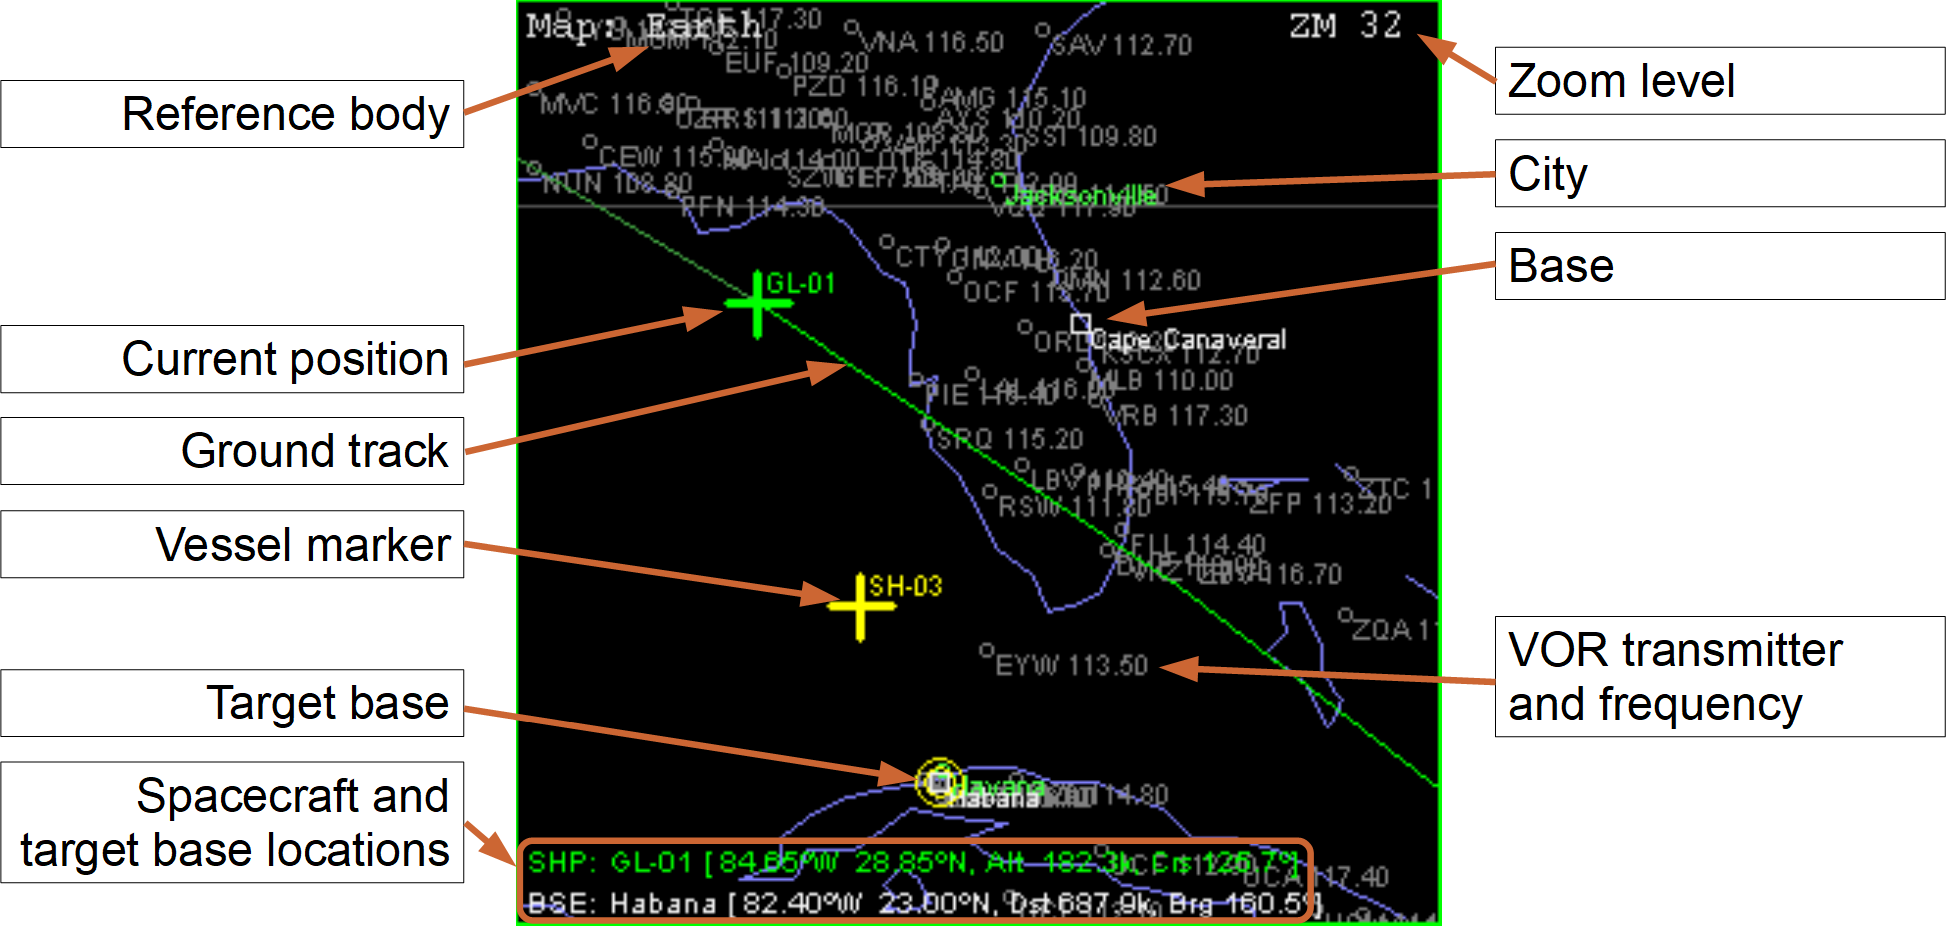
\includegraphics[width=0.99\hsize]{map_layout_2.png}
\end{figure}

\noindent
Display options can be selected from the configuration page (DSP, \Shift\keystroke{D}). Select an item with the UP (\Shift\keystroke{-}) and DN (\Shift\keystroke{=}) buttons, then cycle its settings with MOD (\Shift\keystroke{M}). Return to the map screen with OK (\Shift\keystroke{O}).

\begin{figure}[H]
  \centering
  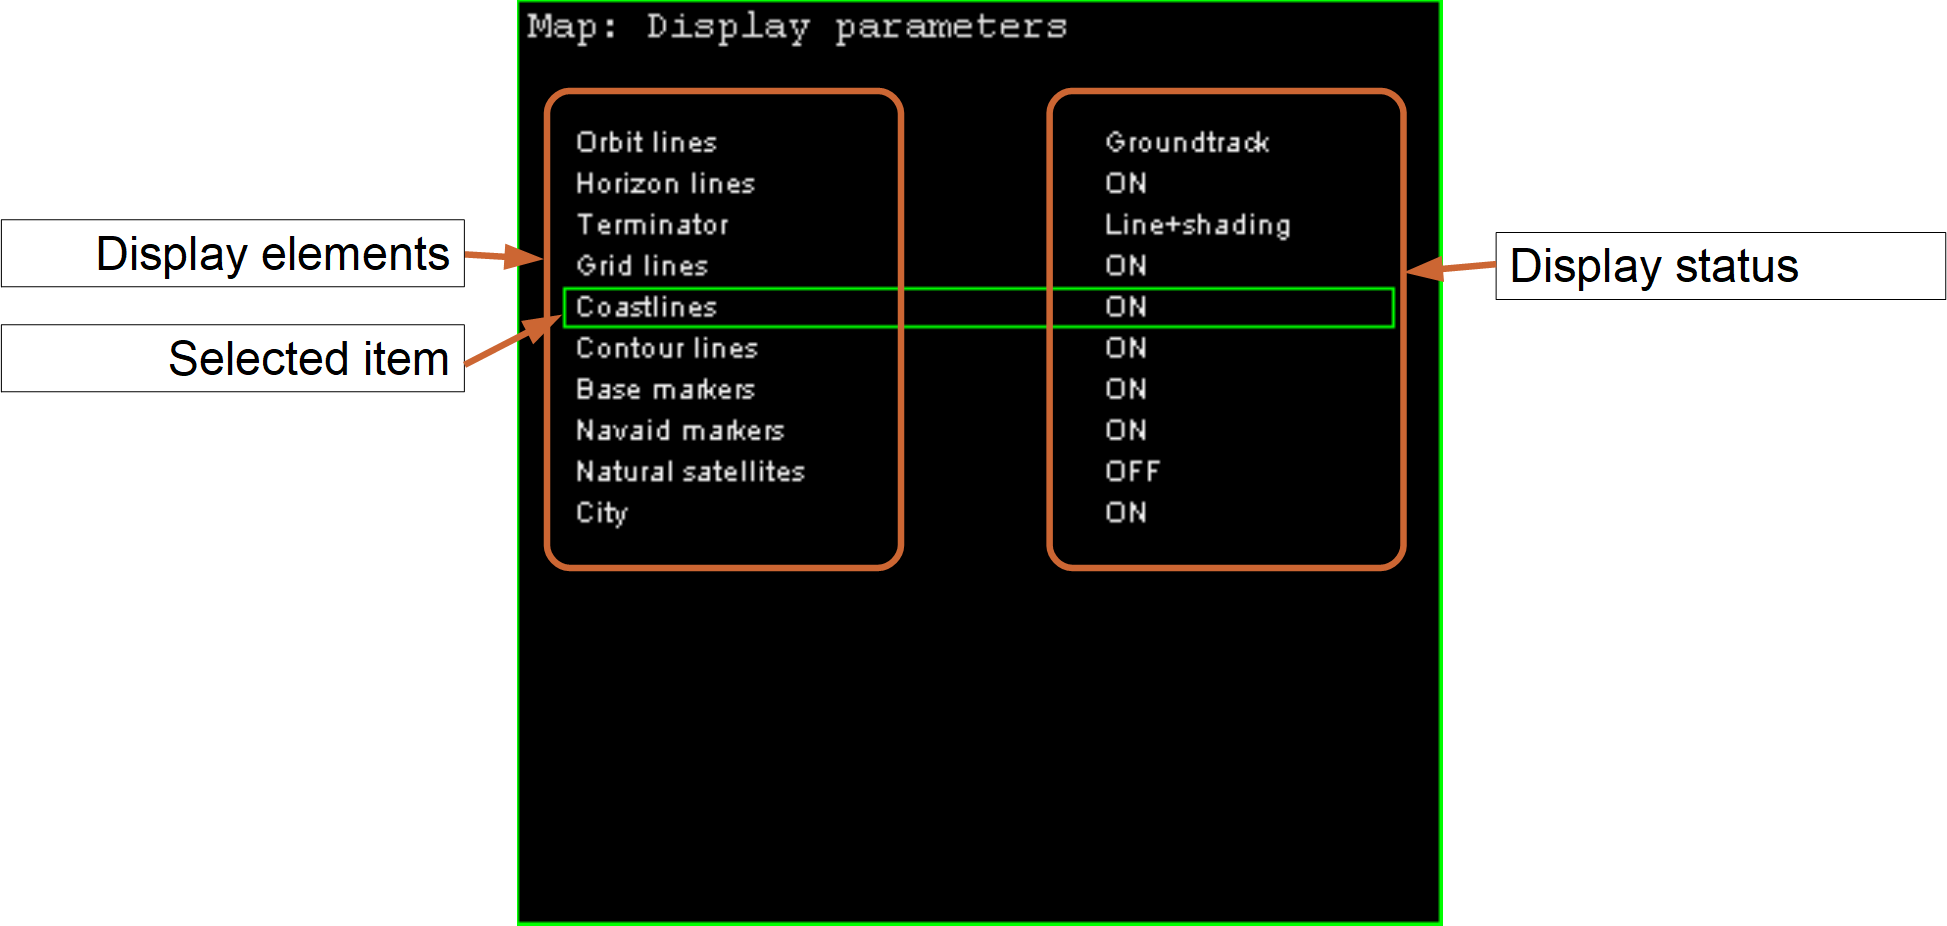
\includegraphics[width=0.99\hsize]{map_params.png}
\end{figure}

\begin{itemize}
\item Only objects (ships, stations or moons) orbiting the displayed celestial body will be accepted as orbit targets. Likewise, only surface bases located on the body will be accepted as target bases.
\item Your ship’s orbital plane will only be plotted if you are orbiting the displayed body.
\end{itemize}


\subsection{VOR/VTOL}
% TODO

\subsection{Horizontal Situation Indicator}
% TODO

\subsection{Orbit}
% TODO

\subsection{Align Orbital Plane}
% TODO

\subsection{Synchronise orbit}
% TODO

\subsection{Docking}
% TODO

\subsection{RCS Attitude}
% TODO

\subsection{Transfer}
% TODO

\end{document}
